\chapter{Аналитический раздел}
\label{cha:analysis}
\section{Анализ предметной области}
Сегодня невозможно представить нашу жизнь без интернета и информационных технологий. Они прочно вошли в нашу жизнь, значительно упростив ее. С развитием информационных технологий нам становятся доступны новые инструменты, которые делают привычные нам процессы удобнее и быстрее, например: покупка товаров, оплата счетов, развлечения и многое другое. Наблюдается стремительный ростом пользователей сети Интернет и объемов информации. Такое стремительное развитие в первую очередь отражается на интернет-провайдерах.

Интернет-провайдер - организация, предоставляющая услуги доступа к сети Интернет и иные услуги. На рисунке~\ref{pic:user_connection_schema} представлена стандартная схема подключения пользователей к сети провайдера.
\begin{figure}
\centering
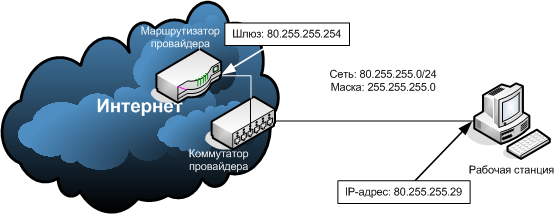
\includegraphics[scale=0.7]{pictures/user_connection_schema}
\caption{Подключение пользователя к сети Интернет}
\label{pic:user_connection_schema}
\end{figure}

В зависимости от видов предоставляемых услуг провайдеры деляется на:
\begin{itemize}
\item провайдеры доступа;
\item хостинг-провайдеры;
\itemмагистральные провайдеры;
\item канальные провайдеры;
\item провайдеры последней мили;
\end{itemize}

Независимо от того, к какой категории относятся провайдеры, они должны обеспечивать бесперебойную, надежную и высокоскоростную передачу данных абонентам. Данные задачи решаются такими методами, как:
\begin{itemize}
\item дублирование информации с целью минимизации расстояния между источником и потребителем;
\item увеличение пропускной способности каналов передачи данных;
\item приоритизация трафика и динамическое управление;
\end{itemize}

Подход, связанный с дублированием (репликацией) информации, активно используется на серверах баз данных. Является дорогим, так как требует дополнительных финансовых расходов, связанных с закупкой оборудования для хранения копий. Также требуется постоянная синхронизация данных между копиями для достижения консистентности данных.

Второй подход также связан с изменение сетевой инфраструктуры - модернизация каналов передачи данных с целью увеличения пропускной способность. Достигается за счет использования более быстрых способов коммутации, например оптоволокна. Аналогично первому подходу является дорогим.

Данная работа посвящена третьему подходу, связанному с приоритизацией и динамическим управлением трафиком. Основная идея заключается в классификации трафика по каким-то критериям и обработке разными способами. На рисунке \ref{pic:qos_simple_example} приведен пример использования классификации трафика для реализации QoS - качества обслуживания. Маршрутизатор 1 настроен таким образом, чтобы выделить до 5 МБит/с из доступных 10 МБит/с передаче потокового видео. Передаче данных по FTP разрешено использовать 2МБит/с, а HTTP и другому трафику до 3 МБит/с.
\begin{figure}
\centering
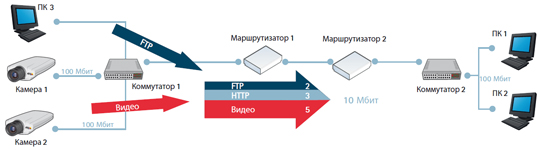
\includegraphics[scale=0.7]{pictures/qos_simple_example}
\caption{Пример динамического управления трафиком}
\label{pic:qos_simple_example}
\end{figure}

\subsection{Сетевая модель OSI и стек протоколов TCP/IP}
Сетевая модель OSI - базовая эталонная модель взаимодействия открытых систем. Назначение модели OSI состоит в обобщенном представлении средств сетевого взаимодействия, она разрабатывалась в качестве универсального языка сетевых специалистов, поэтому ее называют справочной моделью.

В связи с затянувшейся разработкой протоколов OSI, в настоящее время основным стеком протоколов является TCP/IP. Протоколы работают друг с другом в стеке - это означает, что протокол, располагающийся на уровне выше, работает
"поверх" нижнего, используя механизмы инкапсуляции. На рисунке~\ref{pic:model_osi_vs_tcpip} приведены обе модели, а также показаны их основные различия.
\begin{figure}[h]
\centering
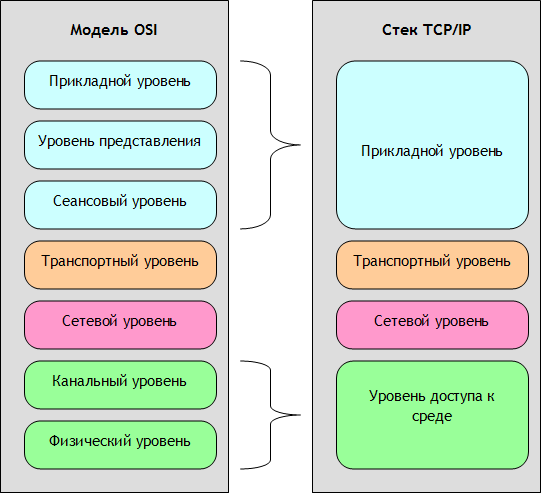
\includegraphics[scale=0.5]{pictures/model_osi_vs_tcpip}
\caption{Модель OSI и TCP/IP}
\label{pic:model_osi_vs_tcpip}
\end{figure}

На канальном уровне в большинстве сетей используется семейство технологий пакетной передачи данных Ethernet. В зависимости от скорости передачи данных, и передающей среды, существует несколько вариантов технологии:
\begin{itemize}
\item ранние модификации Ethernet;
\item 10 МБит/с Ethernet;
\item Быстрый Ethernet (Fast Ethernet, 100 МБит/с);
\item Гигабитный Ethernet (Gigabit Ethernet, 1 ГБит/с);
\item 2.5 и 5-гигабитные варианты (NBASE-T, MGBASE-T);
\item 10-гигабитный Ethernet (10G Ethernet, 10 ГБит/с);
\item 40-гигабитный и 100-гигабитный Ethernet;
\end{itemize}

Разрабатываемый сетевой сервис будет работать только с Ethernet-картами любых скоростей, при этом другие технологии канального уровня не поддерживаются.

\subsection{Технология DPI}
Анализ пакетов является важной задачей не только для классификации трафика, но и для всего функционирования сети. Любой сетевой коммутатор вынужден просматривать каждый пакет с целью изучения его mac-адреса отправителя и получателя. Эта информация нужна ему для того, что определить в какой выходной порт отправить пакет. Сетевые маршрутизаторы просматривают ip-адреса отправителя и получателя (если речь идет о TCP/IP-сетях) и в дальнейшем строят таблицы маршрутизации.

В наше время провайдеры сталкиваются с проблемами, которые не могут решиться только анализом заголовков пакетов, например:
\begin{itemize}
\item высокая загрузка канала к пользователю (скачивание Bittorent);
\item высокая нагрузка на каналы провайдера (все пользователи скачиваю Bittorent);
\item большая часть пропускной способности занимается наименьшей частью наиболее активных абонентов;
\item атаки на оборудование, вирусы, боты;
\end{itemize}

Для решения всех этих проблем может применяться технология DPI (глубокой анализ пакетов) - технология накопления статистических данных, проверки и фильтрации сетевых пакетов по их содержимому. Ключевая идея состоит в том, чтобы анализировать не только заголовки пакетов, такие как Ethernet, IP, TCP или UDP, но и остальные данные пакета с целью выявления определенных сигнатур или других особенностей, присущих искомому трафику. Самыми распространенными способами реализации DPI являются статический анализ и анализ косвенных признаков, присущих определенным протоколам. 

Система DPI, как правило, устанавливается на границе сети провайдера в разрыв существующих каналов, уходящих в пограничные маршрутизаторы, тем самым весь трафик, который покидает или входит в сеть оператора проходит через DPI, что дает возможность его мониторинга и контроля. В отдельных случаях можно устанавливать эту систему не на границе сети, а спускать ее ближе к конечным пользователям, но из экономических соображений так делают редко.

На рынке DPI есть модели от различных вендоров по различным ценам, все зависит от производительности и списка возможностей. Все они, как правило, реализуются в составе с высокопроизводительными системами. В данной работе рассматривается чисто программная реализация технологии DPI под архитектуру процессоров $x86_64$.


\section{QoS и DPI}
С точки зрения эксплуатации, провайдер может контролировать утилизацию подключенных через DPI каналов на уровне приложений. Раньше задача реализации QoS решалась исключительно средствами построения очередей на основании маркировки трафика служебными битами в заголовках IP, а также используя VLAN или MPLS метки, выделяя наиболее приоритетный трафик и гарантируя ему определенную пропускную способность в любой момент времени. При этом весь трафик домашних абонентов оставался без контроля, что давало возможность трафику Bittorent забрать себе всю свободную полосу.

С использованием DPI у провайдера появляется возможность распределить канал между различными приложениями, так, например, можно разрешить в ночные часы Bittorent с большей пропускной способностью, чем днем, когда в сети находится большое количество другого трафика.


\section{Межсетевой экран}
Межсетевой экран - комплекс аппаратных и программных средств в компьютерной сети, осуществляющий контроль и фильтрацию проходящих через него сетевых пакетов в соответствии с заданными правилами. Основной задачей сетевого экрана является защита сети или отдельных ее узлов от несанкционированного доступа, осуществление трансляции адресов - динамическую замену внутрисетевых (серых) адресов или портов на внешние, используемые за пределами локальной сети.

Различают следующие типы межсетевых экранов:
\begin{itemize}
\item управляемые коммутаторы (канальный уровень);
\item сетевые фильтры (сетевой уровень, анализ ip-адресов);
\item шлюзы сеансового уровня;
\item шлюз прикладного уровня (прокси-сервера);
\end{itemize}

В ядре Linux есть межсетевой экран под названием Netfilter, встроен в ядро с версии 2.4. Основным инструментов управления является Iptables - утилита командной строки, с ее помощью администраторы создают и изменяют правила, управляющие фильтрацией и перенаправлением пакетов.

В системе Netfilter пакеты пропускаются через цепочки. Цепочка является упорядоченным списком правил, а каждое правило может содержать критерии, действие или переход. Когда пакет проходит через цепочку, система по очереди проверяет, соответствует ли пакет всем критериям очередного правила, и если так, то выполняет действие. Набор критериев в системе Netfilter ограничен только заголовками протоколов и никак не учитывает остальную часть пакета, что является главным недостатком и не допускает использование Netfilter в сетях провайдера.

Существуют расширенные версии Netfilter, позволяющие выполнять более детальную проверку пакетов. Все они являются узкоспециализированными и реализуются, в основном, патчами ядра Linux, что предполагает перекомпиляцию самого ядра. Такое решение является непрактичным и используется редко.

Технология DPI идеально подходит для реализации функций межсетевого экрана, так как выполняет полный анализ пакета. Главным преимуществом является возможность контролировать информацию на прикладном уровне и классифицировать сотни протоколов без привязки к конкретному порту TCP или UDP. Благодаря этому можно, к примеру, блокировать Skype-трафик, а также любые виды SIP-телефонии.

Разрабатываемый сервис будет выполнять функции сетевого экрана и поддерживать анализ следующих протоколов:
\begin{itemize}
\item SIP
\item RTP
\item RTSP
\item HTTP
\end{itemize}


\section{Балансировка трафика}

\subsection{MPLS-сети}

\subsection{VLAN-сети}


\section{Обзор существующих решений}

\subsection{Проет OpenDPI}

\subsection{Проект nDPI}

\section{Постановка задачи}
